\documentclass[12pt]{article}
%\usepackage[a4paper, total={6in, 10in}]{geometry}
\usepackage[top=0in, bottom=1in, left=1.25in, right=1.25in]{geometry}



\usepackage{graphicx}
\graphicspath{{figs/}} 


\title{Analysing Complexity of Movement Variability 
for Facial Expressions with Nonlinear Dynamics} 
\author{Miguel Xochicale\\ 
}
\date{21th December 2018}

\begin{document}
\maketitle
%\thispagestyle{empty} %No number


%\begin{abstract}
%
%\end{abstract}


\section{Introduction}
Movement variability is an inherent feature within and between persons. 
Research on measurement and understanding of movement variability has been 
well established in the last three decades in areas such as biomechanics, 
sport science, psychology, cognitive science, neuroscience and robotics 
\cite{2018arXiv181009249X}.
Also, considering that methodologies for movement variability 
to quantify variability in facial expressions and 
my preliminary experiments of the analysis of variations 
for facial expressions using nonlinear dynamics \cite{MPXochicale_CERE2018}.
I am interested in quantifying the complexity 
of facial expression that one person or multiple persons can present in scenarios 
of human-robot interaction and  in researching 
the subtle variations of facial expressions that are related to different 
mental states  (e.g. anxiety, disinterest, relief) \cite{back2014}.
Hence, such statements have led me to ask two questions in the context
of human-robot interaction: 
(i) does the quantification of the variation for facial expressions 
using nonlinear dynamics can tell us something about the state of mind of a person?, 
(ii) how the quantification of facial expressions can be related with 
the complexity of facial expressions?.

\section{Methods}
Considering the work in my Ph.D. thesis where investigated nonlinear dynamics
to quantify movement variability \cite{XochicalePhDThesis2018},
I am proposing to apply Recurrence Quantification Analysis (RQA) for this work.
RQA computes measurements based on the recurrence points density of diagonal 
or vertical line structures in Recurrence Plots. 
Such measurements of dynamics can determine the dynamics of a system,
e.g. the determinism (predictability) or Shannon entropy (complexity) 
\cite{marwan2007}. 
Hence, the use Shannon Entropy can be applied to measure 
from the recurrent quantification analysis (also known as RQAEntr)
to quantify the complexity of face expressions. 


\section{Preliminary results}


Fig \ref{fig:method} shows the proposed methodology with 
some preliminary results of one participant performing three
levels of face expressions. 


%%---------------------------------(FIGURE)-------------------------------------
\begin{figure}
\centering
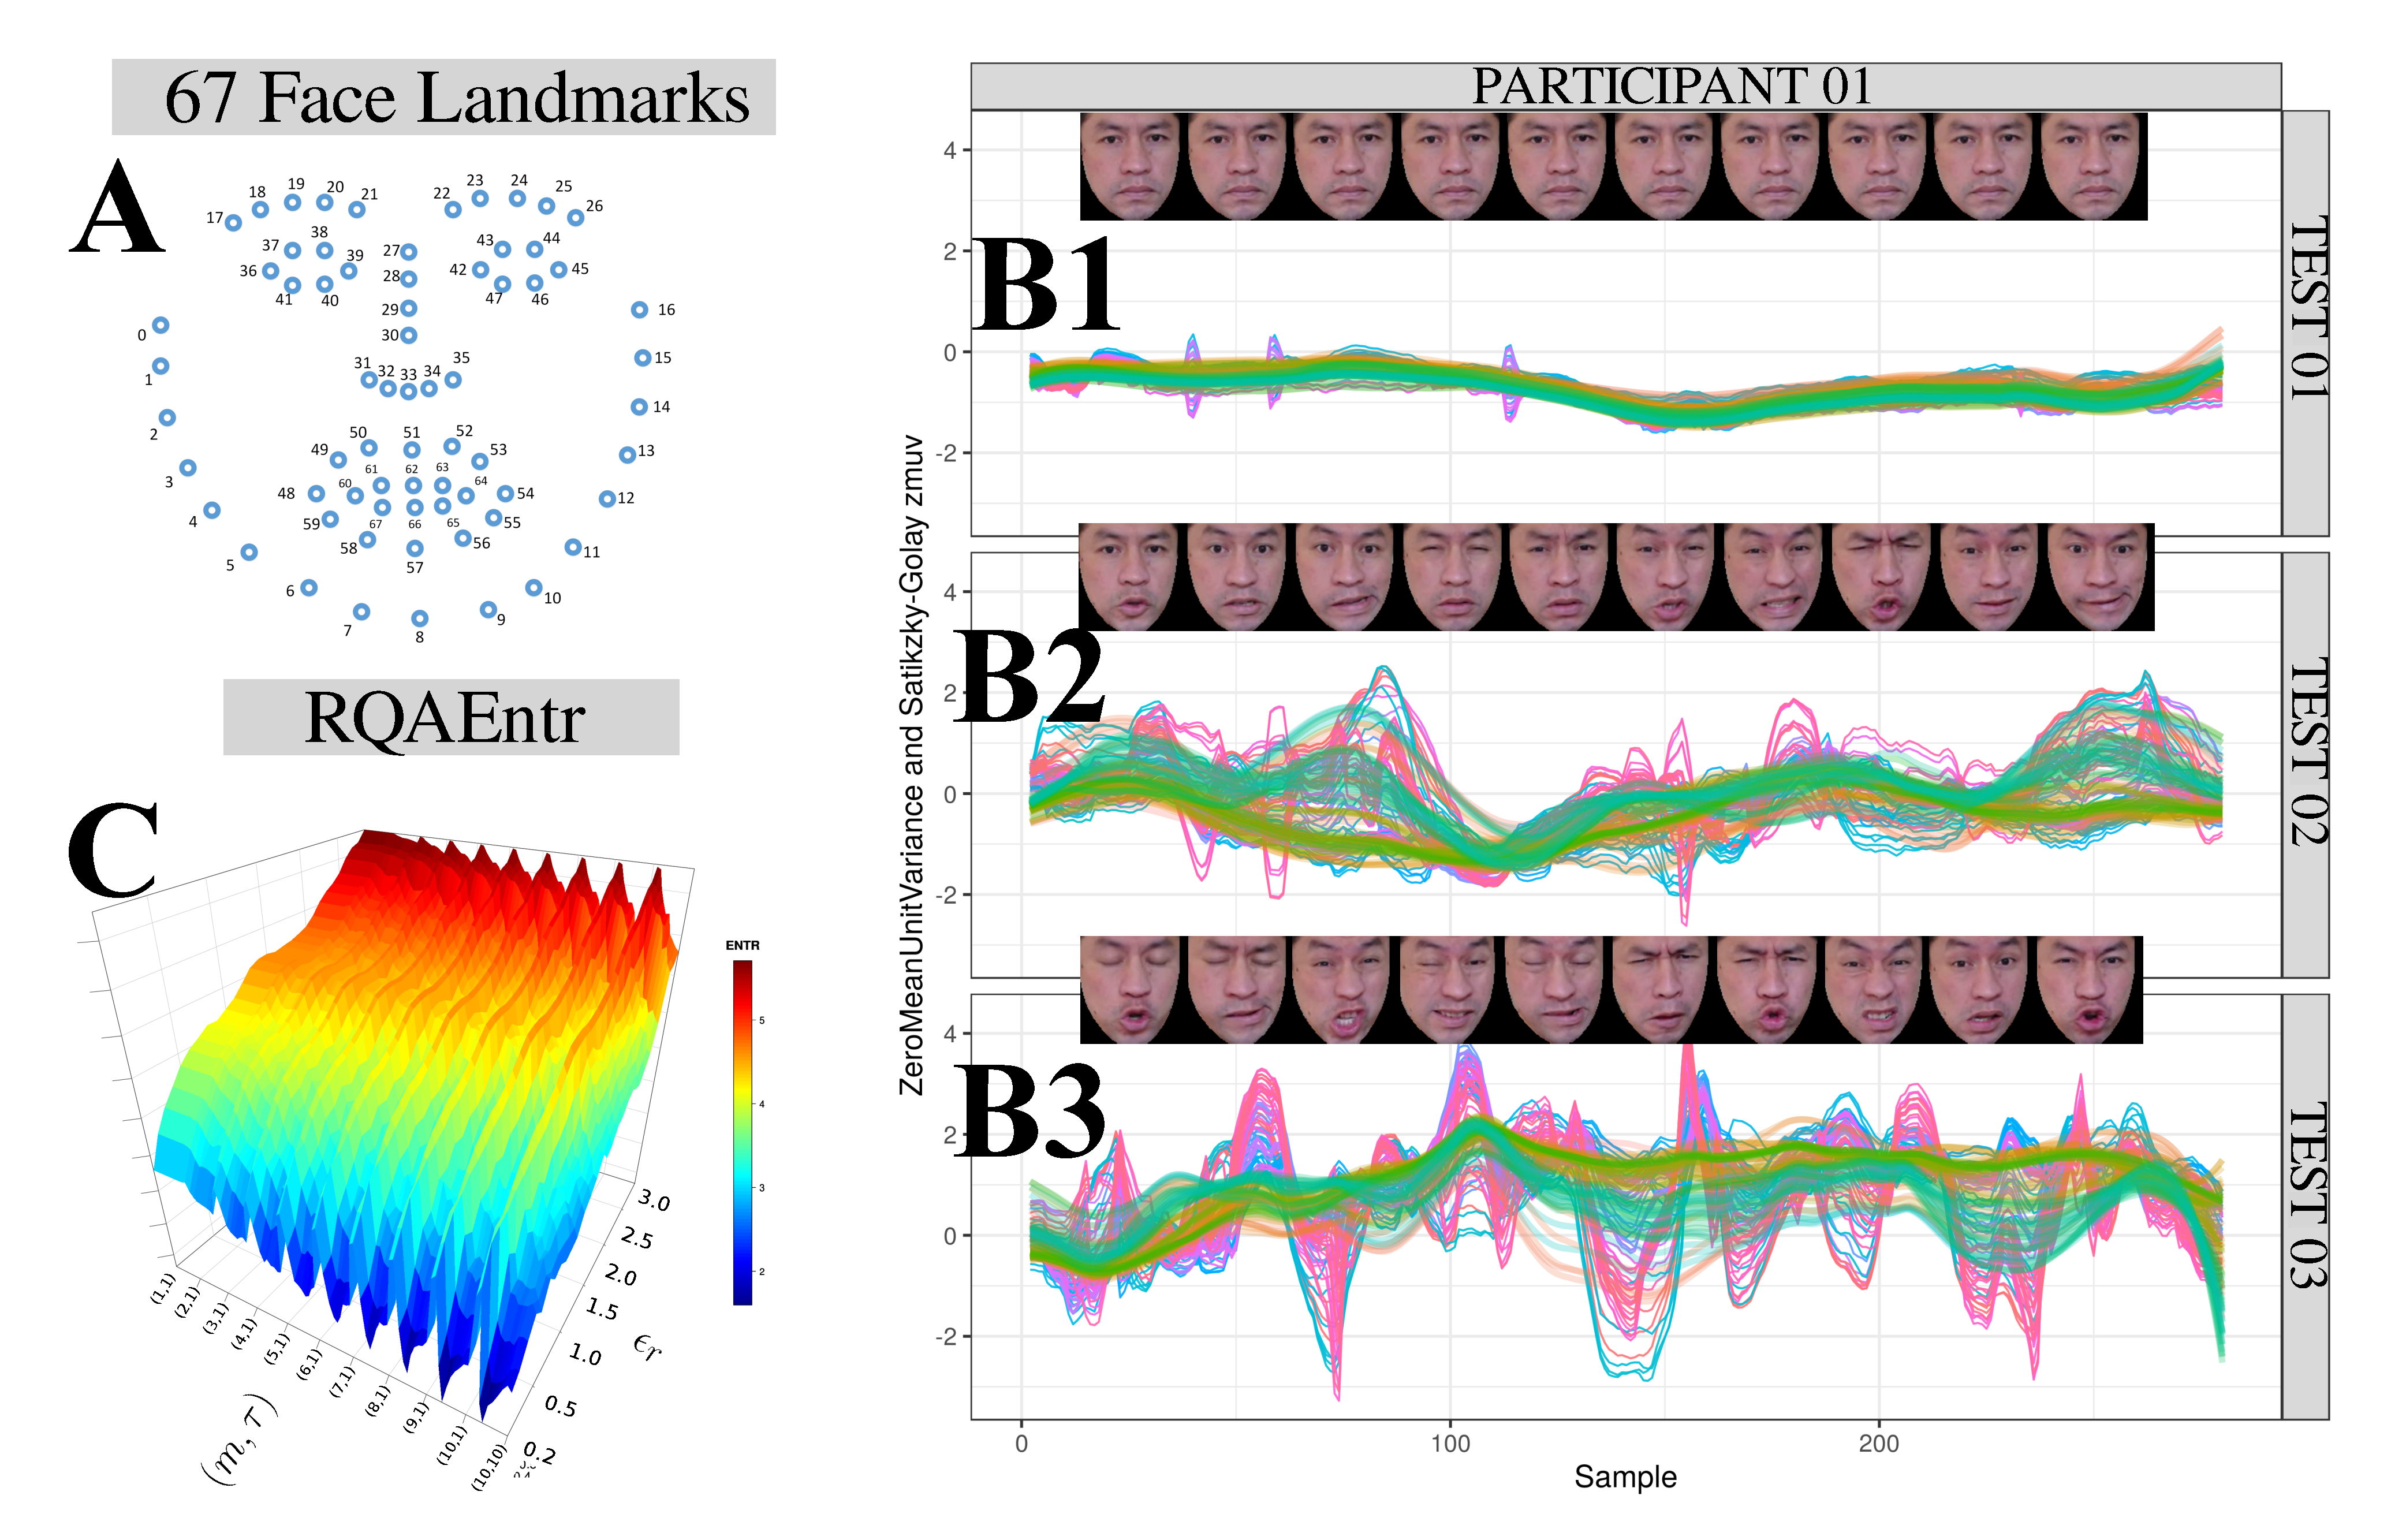
\includegraphics[width=1.0\textwidth]{main/method}
    \caption{
	{\bf Quantifying variations of face variations using nonlinear dynamics.}
	(A) Head pose estimation and face landmarks with OpenFace \cite{baltrusaitis2018},
	(B) time series from landmarks, and
	(C) 3D surface of RQAEntr for one time series.
        }
\label{fig:method}
\end{figure}
%%---------------------------------(FIGURE)------





%\newpage

\bibliographystyle{apalike}
\bibliography{references/references}


\end{document}
